%!TEX root = ../../main.tex
\section{Small Angle X-ray Scattering (SAXS)}
\label{sec:Small Angle X-ray Scattering}
    Small angle X-ray scattering (SAXS) is a technique used to determine the overall shape and size of a macromolecule, which like X-ray crystallography, requires a sample containing the molecule to be irradiated with a beam of X-rays.
    However, unlike X-ray crystallography, SAXS does not require the growth of crystals.
    Instead, the protein solution is irradiated and the diffracted X-rays are collected on a position sensitive detector.
    In solution, the movement of molecules is not restricted and they can adopt random orientations with respect to one another \cite{blanchet2013small}.
    Therefore the data observed on the detector are not individual Bragg peaks.
    Although SAXS does not provide atomic level detail of a structure, it does give information about the interatomic distances between atoms, as well as an overall envelope of the structure and the molecular weight of the molecule \cite{pollack2011saxs}.

    The X-ray scattering intensity is radially isotropic and hence it is determined by taking a radial average of the intensities recorded on the detector image \cite{franke2015correlation}.
    The radially averaged intensity is usually written as a function of the momentum transfer, $q$, which itself is defined in terms of the scattering angle:
    \begin{equation}
        q = \f{4 \pi \sin(\theta)}{\lambda}
        \label{eq:momentum transfer}
    \end{equation}
    The final scattering pattern is the result of subtracting the radially averaged intensity of the solution containing the protein from the radially averaged intensity of the solution containing the buffer without protein (Figure~\ref{fig:SAXS scattering curve}).
    \begin{figure}
        \centering
        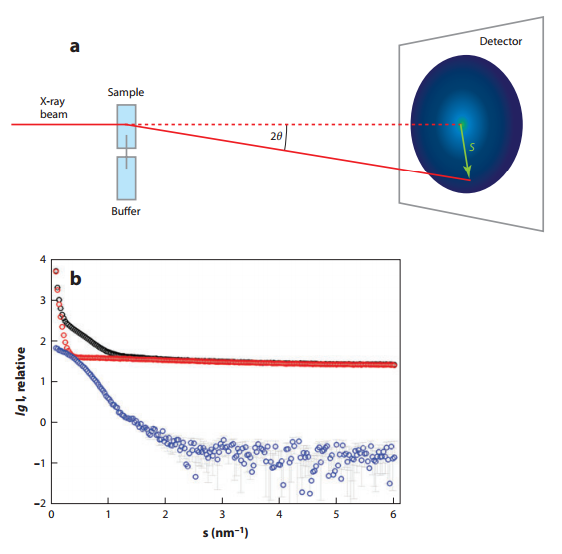
\includegraphics[width=0.8\textwidth]{figures/introduction/SAXS_scattering.png}
        \caption[SAXS data collection schematic and resulting radially averaged intensity curve.]{(a) X-ray beam (typical energies between 7 and 12.5\,keV \cite{hopkins2016quantifying}) is incident on a SAXS sample and the scattered radiation is collected on a detector.
        The symbol $s$ in the figure is equivalent to the momentum transfer denoted $q$ in equation \ref{eq:momentum transfer}.
        (b) Radially averaged intensity curves from a solution of bovine serum albumin (BSA).
        The radially averaged intensity of the solution containing only the buffer (red curve) is subtracted from the radially averaged intensity of the solution containing BSA and buffer (black curve) to obtain the resulting intensity curve for BSA (blue curve) \cite{blanchet2013small}.}
        \label{fig:SAXS scattering curve}
    \end{figure}

    Several graphs are produced during the analysis of SAXS data which can give much information about the state of the protein.
    For example, Kratky plots give indications of whether or not a protein is in a folded state (Figure~\ref{fig:Kratky plot}).
    This is because Debye's equation, (equation \ref{eq:Debye function SAXS}), which describes the scattering intensities, $I_{Gauss}$, for molecules behaving as Gaussian coils, plateaus in a $q^2 \times I(q)$ vs $q$ plot within a limited range of data.
    \begin{equation}
        I_{Gauss}(q) = 2 I_0 \f{\exp(-u) + u -1}{u^2},
        \label{eq:Debye function SAXS}
    \end{equation}
    where $I_0$ is incident X-ray intensity and
    \begin{equation}
        u = q^2 R_g^2,
    \end{equation}
    where $R_g$ is the radius of gyration.

    The Fourier transform of the SAXS pattern gives the pair-distance distribution function, a function that provides information about the interatomic distances in the protein:
    \begin{equation}
        p(r) = \f{r^2}{2\pi^2}\int_0^{\infty}q^2 I(q) \f{\sin(qr)}{qr}\ \mathrm{d}q.
    \end{equation}
    where $r$ is the distance between electrons in the molecule.
    Examples of distance distribution functions for various geometrical shapes are shown in Figure~\ref{fig:Distance distribution plot}.
    \begin{figure}
        \centering
        \begin{subfigure}[b]{0.8\textwidth}
                \centering
                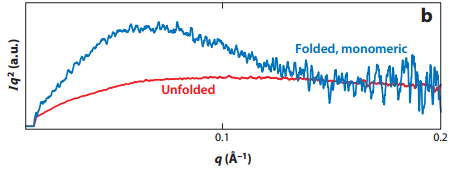
\includegraphics[width=\textwidth]{figures/introduction/kratkyplot.png}
                \caption{}
                \label{fig:Kratky plot}
        \end{subfigure}
        \\
        \begin{subfigure}[b]{0.6\textwidth}
                \centering
                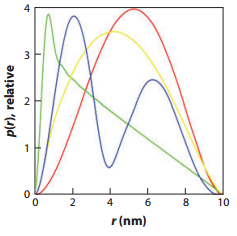
\includegraphics[width=\textwidth]{figures/introduction/distancedistribution.png}
                \caption{}
                \label{fig:Distance distribution plot}
        \end{subfigure}
        \caption[Example Kratky curves and distance distribution function]{(a) Kratky plots.
        The red curve shows the unfolded RNA domain P4-P6 from the \textit{Tetrahymena} ribozyme where the salt concentration was low.
        The blue curve implies the domain was folded and monomeric \cite{pollack2011saxs}.
        (b) Distance distribution functions for several geometrical volumes: sphere (red),  dumbbell (blue), cylinder (green) disk (yellow) \cite{blanchet2013small}.}
        \label{fig:SAXS structural analysis graphs}
    \end{figure}
